\PassOptionsToPackage{unicode=true}{hyperref} % options for packages loaded elsewhere
\PassOptionsToPackage{hyphens}{url}
%
\documentclass[]{article}
\usepackage{lmodern}
\usepackage{amssymb,amsmath}
\usepackage{ifxetex,ifluatex}
\usepackage{fixltx2e} % provides \textsubscript
\ifnum 0\ifxetex 1\fi\ifluatex 1\fi=0 % if pdftex
  \usepackage[T1]{fontenc}
  \usepackage[utf8]{inputenc}
  \usepackage{textcomp} % provides euro and other symbols
\else % if luatex or xelatex
  \usepackage{unicode-math}
  \defaultfontfeatures{Ligatures=TeX,Scale=MatchLowercase}
\fi
% use upquote if available, for straight quotes in verbatim environments
\IfFileExists{upquote.sty}{\usepackage{upquote}}{}
% use microtype if available
\IfFileExists{microtype.sty}{%
\usepackage[]{microtype}
\UseMicrotypeSet[protrusion]{basicmath} % disable protrusion for tt fonts
}{}
\IfFileExists{parskip.sty}{%
\usepackage{parskip}
}{% else
\setlength{\parindent}{0pt}
\setlength{\parskip}{6pt plus 2pt minus 1pt}
}
\usepackage{hyperref}
\hypersetup{
            pdftitle={Tables for SAPFLUXNET data paper},
            pdfauthor={R. Poyatos},
            pdfborder={0 0 0},
            breaklinks=true}
\urlstyle{same}  % don't use monospace font for urls
\usepackage[margin=1in]{geometry}
\usepackage{graphicx,grffile}
\makeatletter
\def\maxwidth{\ifdim\Gin@nat@width>\linewidth\linewidth\else\Gin@nat@width\fi}
\def\maxheight{\ifdim\Gin@nat@height>\textheight\textheight\else\Gin@nat@height\fi}
\makeatother
% Scale images if necessary, so that they will not overflow the page
% margins by default, and it is still possible to overwrite the defaults
% using explicit options in \includegraphics[width, height, ...]{}
\setkeys{Gin}{width=\maxwidth,height=\maxheight,keepaspectratio}
\setlength{\emergencystretch}{3em}  % prevent overfull lines
\providecommand{\tightlist}{%
  \setlength{\itemsep}{0pt}\setlength{\parskip}{0pt}}
\setcounter{secnumdepth}{0}
% Redefines (sub)paragraphs to behave more like sections
\ifx\paragraph\undefined\else
\let\oldparagraph\paragraph
\renewcommand{\paragraph}[1]{\oldparagraph{#1}\mbox{}}
\fi
\ifx\subparagraph\undefined\else
\let\oldsubparagraph\subparagraph
\renewcommand{\subparagraph}[1]{\oldsubparagraph{#1}\mbox{}}
\fi

% set default figure placement to htbp
\makeatletter
\def\fps@figure{htbp}
\makeatother


\title{Tables for SAPFLUXNET data paper}
\author{R. Poyatos}
\date{9th January 2020}

\begin{document}
\maketitle

\hypertarget{contents}{%
\subsection{Contents}\label{contents}}

\hypertarget{figure-s1.}{%
\subsubsection{Figure S1.}\label{figure-s1.}}

QC overview, showing file management, identifying automatic and manual
steps and indicating status file updates. \#\#\# Table S1. Quality
control of metadata in the QC1 stage. \#\#\# Figure S2. Structure of
sfn\_data objects. \#\#\# Table S2. Metadata variables of SAPFLUXNET
datasets. \#\#\# Table S3. Quality control of metadata in the QC2 stage.
\#\#\# Figure S3. Example of the interactive application for outlier and
and out of range detection in the QC2 stage. \#\#\# Table. Datasets
\#\#\# Table. Number of trees per genus \#\#\# Table. Number of trees
per species

\pagebreak

\hypertarget{supplementary}{%
\subsection{Supplementary}\label{supplementary}}

\pagebreak

\begin{figure}

{\centering 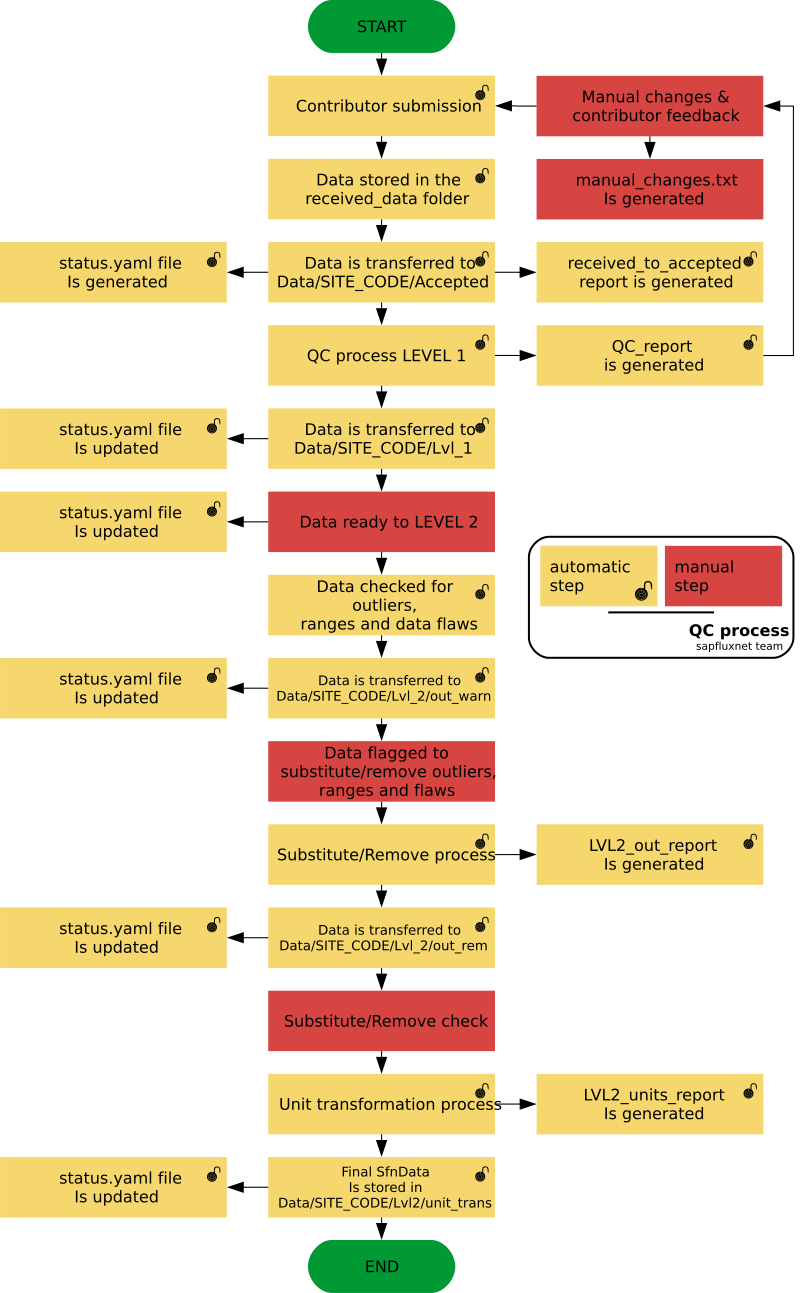
\includegraphics[height=800px]{resources/QC_summary2} 

}

\caption{Figure S1. Overview of the data QC process}\label{fig:fig_QC}
\end{figure}

\pagebreak

\includegraphics[width=6.80in,height=8.02in,keepaspectratio]{supporting_files/figure-latex/table_QC1-1.png}
\pagebreak

\begin{figure}

{\centering 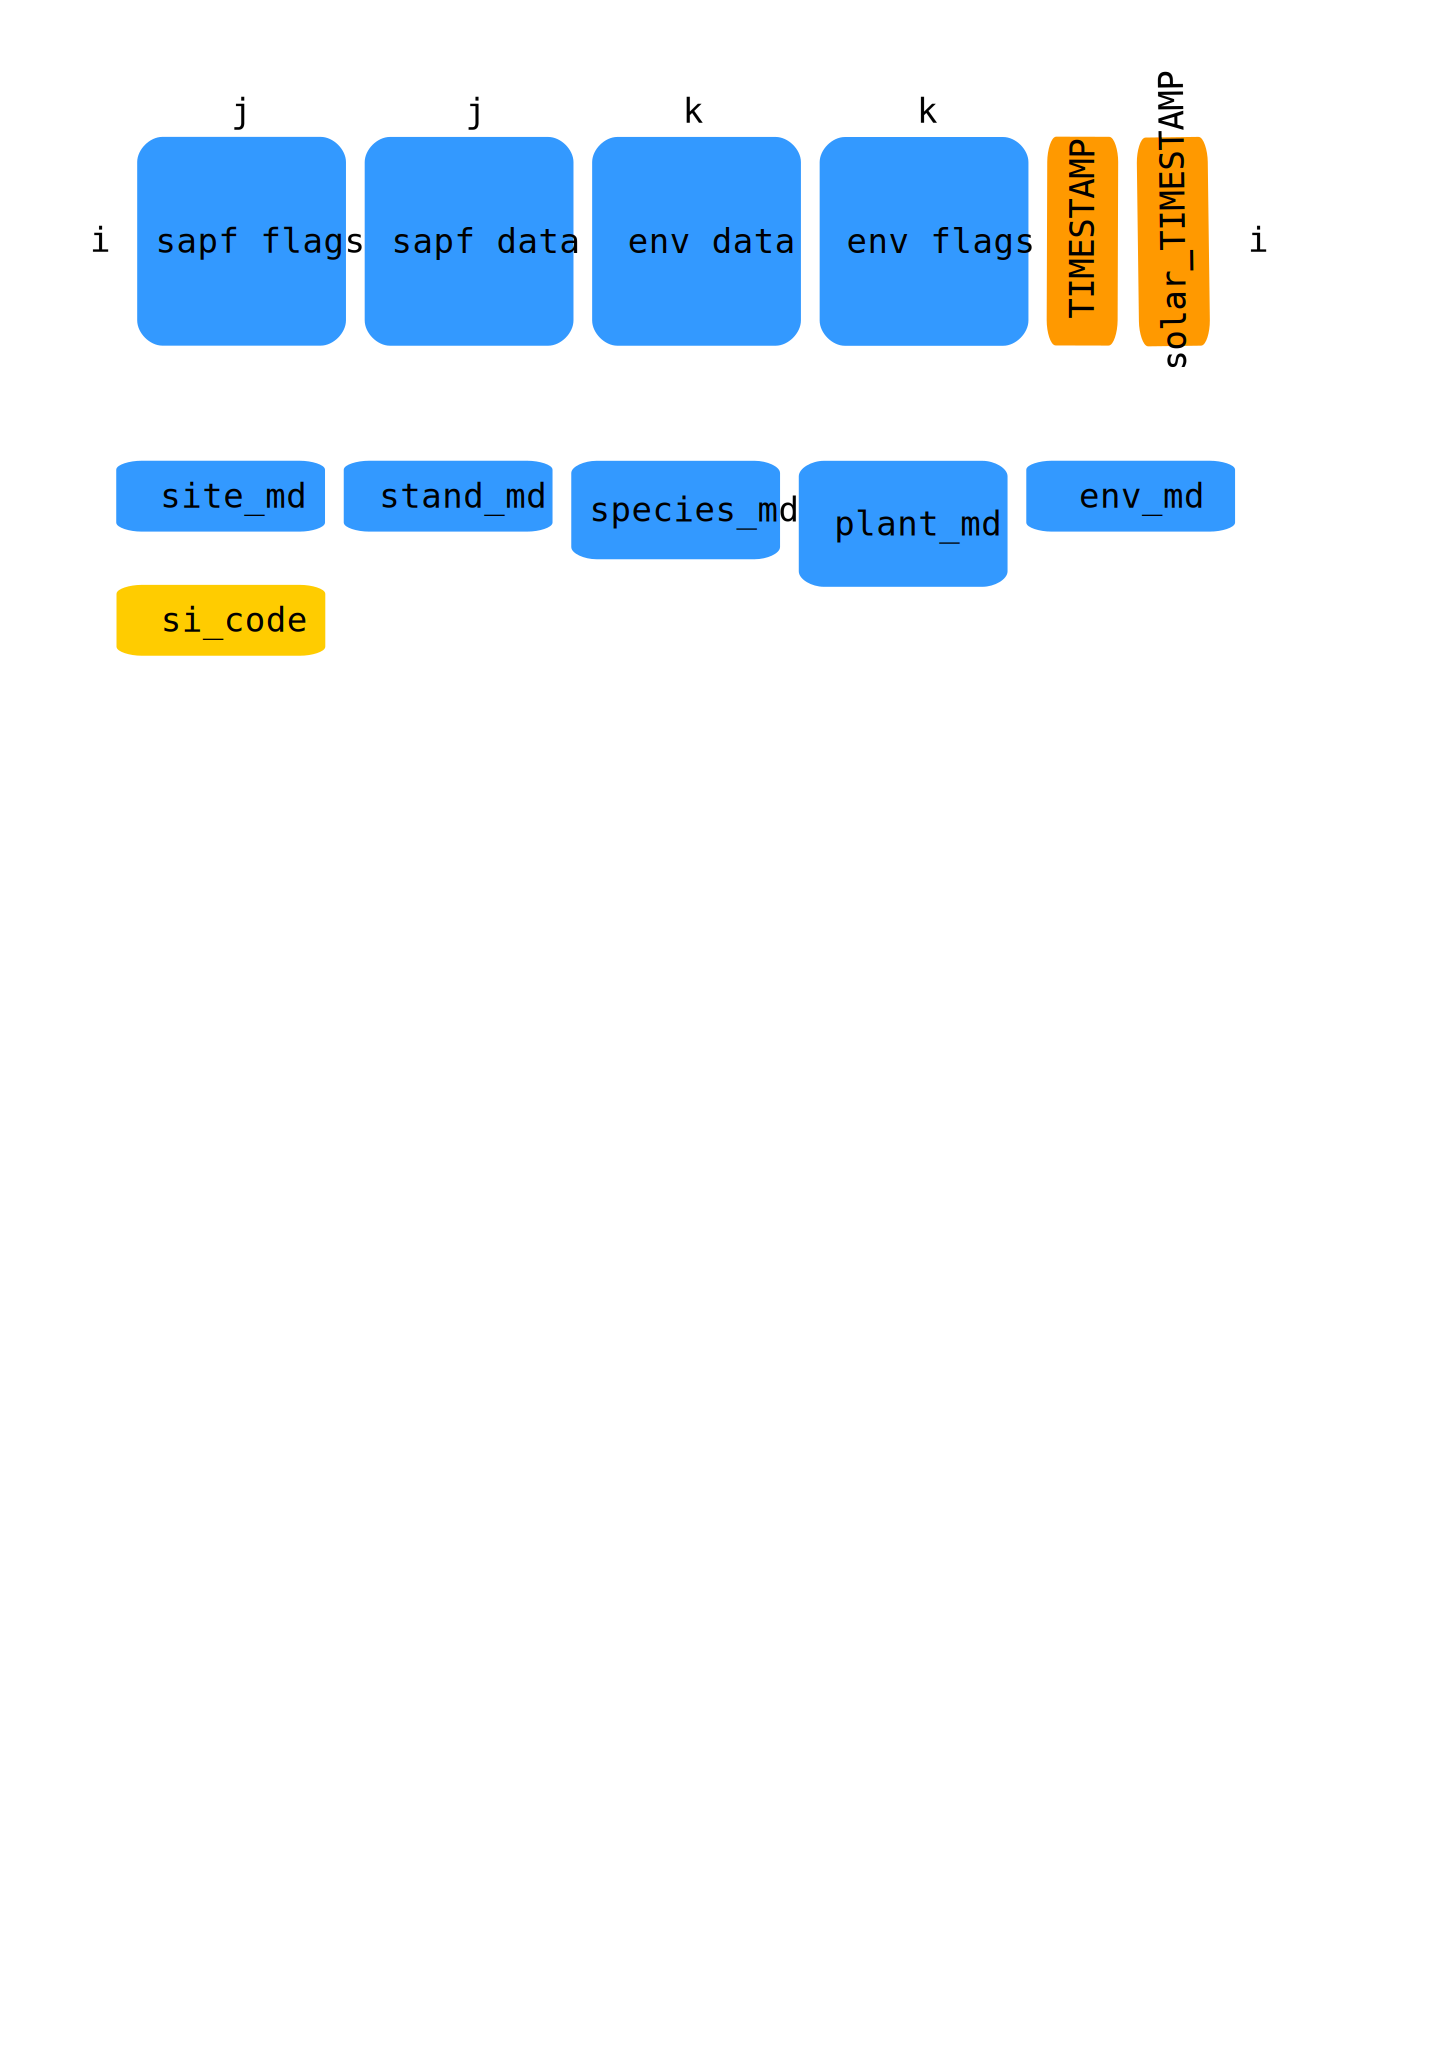
\includegraphics[height=800px]{resources/schematics} 

}

\caption{Figure X. Overview of the data QC process}\label{fig:fig_sfn_data}
\end{figure}

\pagebreak

\includegraphics[width=6.45in,height=76.82in,keepaspectratio]{supporting_files/figure-latex/tab_metadatavars-1.png}
\pagebreak

\begin{figure}

{\centering 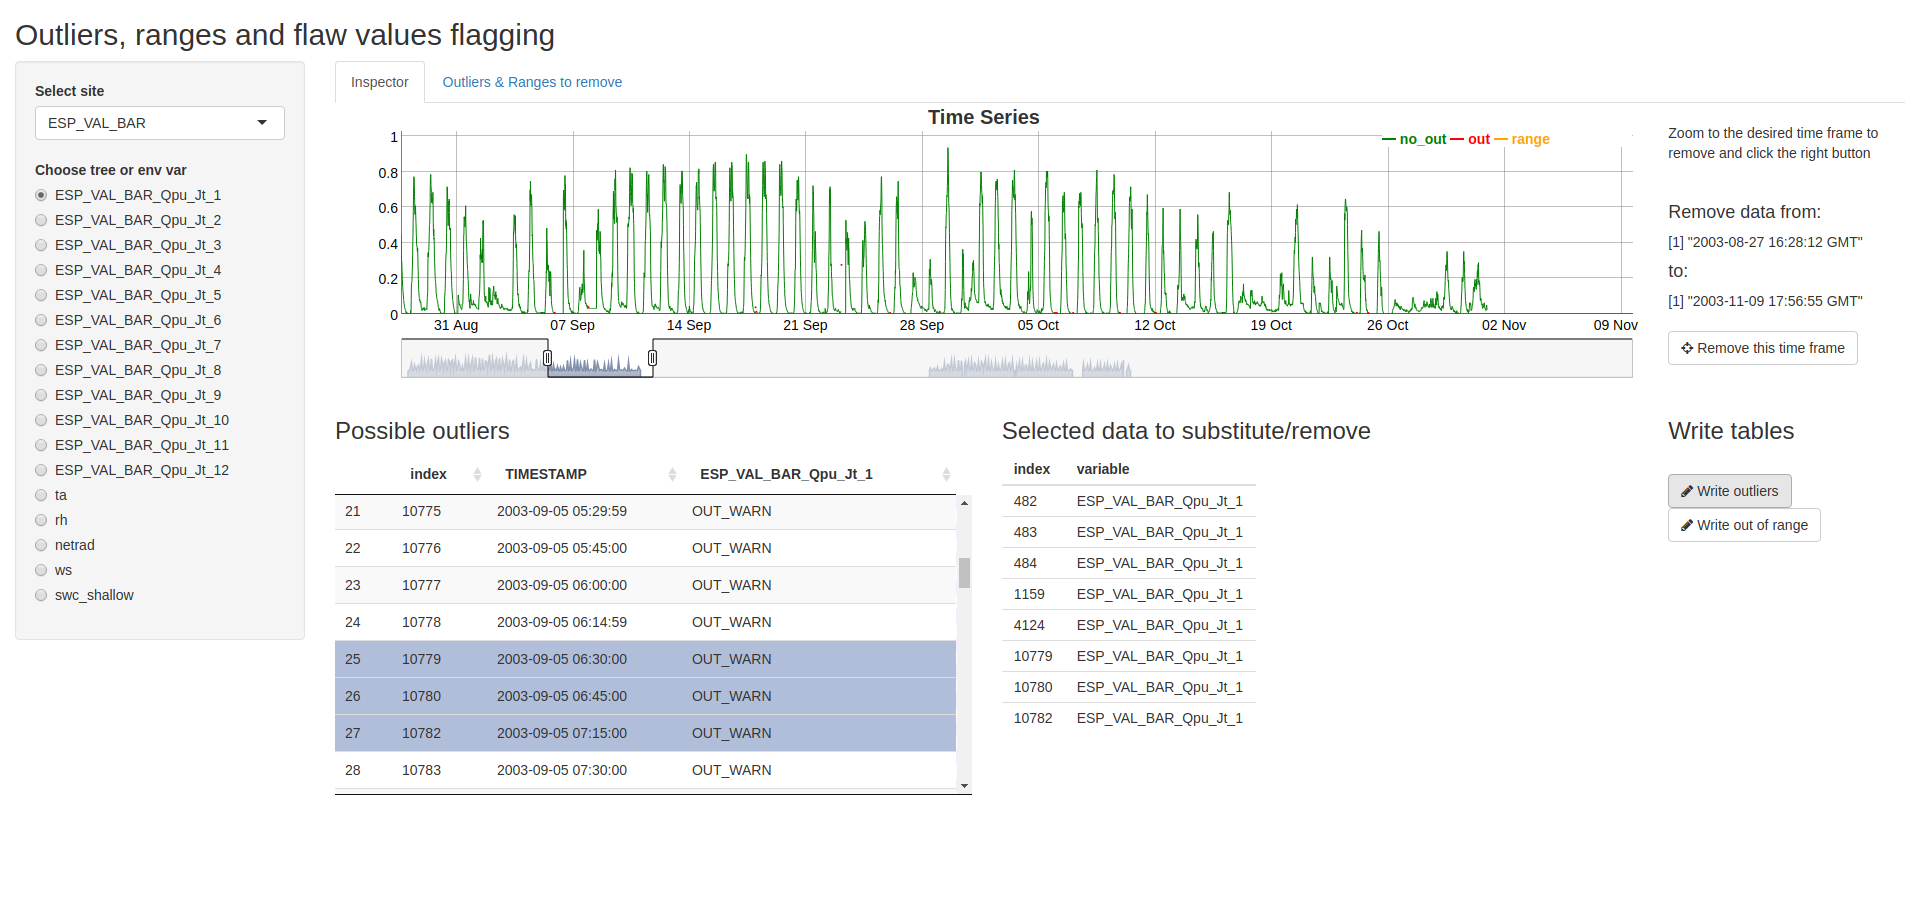
\includegraphics[width=26.67in,height=800px]{resources/out_app} 

}

\caption{Figure SX. Outliers app}\label{fig:fig_outliers_app}
\end{figure}
\pagebreak

\includegraphics[width=7.51in,height=63.13in,keepaspectratio]{supporting_files/figure-latex/tab_sites-1.png}

\pagebreak

\includegraphics[width=9.20in,height=12.71in,keepaspectratio]{supporting_files/figure-latex/tab_ntrees_species-1.png}

\pagebreak

\includegraphics[width=6.00in,height=7.00in,keepaspectratio]{supporting_files/figure-latex/tab_ntrees_genus-1.png}
\pagebreak

\includegraphics[width=9.16in,height=12.72in,keepaspectratio]{supporting_files/figure-latex/tab_nspecies_dataset-1.png}
\pagebreak

\end{document}
